\section{Introduction}
\textit{Biodiversity has declined by more than a quarter in the last 35 years}\footnote{WWF on threats to biodiversity: \url{http://wwf.panda.org/about_our_earth/biodiversity/threatsto_biodiversity/}, Accessed 28-03-2018}. It is estimated that the current extinction rate is between 1,000 and 10,000 times higher than the natural extinction rate due to the interference of humans. It is estimated that between 0.01 and 0.1 percent of all species are going extinct every year\footnote{WWF on species loss: \url{http://wwf.panda.org/about_our_earth/biodiversity/biodiversity/}, Accessed 29-03-2018}.

The biggest contributor to biodiversity loss is \textit{habitat destruction}. The second biggest threat is over-exploitation (e.g. hunting, by-catch). One particular part of over-exploitation is wildlife trade\footnote{Influence of pet trade on animal species: \url{https://www.huffingtonpost.com/the-conversation-global/trading-in-extinction-how_b_14636428.html}, Accessed 29-03-2018}\footnote{WWF on illegal trade: \url{http://wwf.panda.org/about_our_earth/species/problems/illegal_trade/}, Accessed 29-03-2018}. Wildlife trades in products such as ivory or tiger skins is currently considered illegal in order to protect the species. However, the World Wildlife Fund (hereafter referred to as WWF) has discovered a global phenomenon where species collected from the wild are declared as \textit{bred in captivity}. Such trades would be registered as legal but with the animals illegally acquired \cite{Nijman2015,TrafficWWF}. Another case of laundering illegal trades is the ivory business in Hong-Kong. Traders claim that it is easy to launder ivory by using the legal stockpile as a front, while at the same time selling poached ivory \cite{Lo2015}. 

There is a growing worldwide concern with regard to the trade of endangered wildlife species. In order to address this concern, the Convention on International Trade in Endangered Species of Wild Fauna and Flora (hereafter referred to as CITES) was founded. CITES\footnote {The Convention on International Trade in Endangered Species of Wild Fauna and Flora: \url{https://www.cites.org/eng/disc/what.php}, Accessed 23-02-2018} is the international agreement between 183 governments that aims to protect specimens of wild animals and plants from extinction through international trade. 

This paper proposes a visualization to create awareness on the legal trading of endangered animal wildlife species. Through interacting with different parameters of the visualization the user is able to perceive how trade has evolved over time and how and where a particular species is traded. Section \ref{relatedwork} starts off by describing related visualizations and their functions. Hereafter, section \ref{concept} explains the concept of the proposed visualization. Section \ref{data} provides a short summary with regard to the CITES dataset and the mapping of the data to the visualization. Section \ref{design} offers an overview of the different design decisions that were made during the design process. Section \ref{science-excel} explains how insight is generated through the proposed visualization. Finally, section \ref{reflection} reflects on the project and the cooperation within the team responsible. 


\section{Related Visualizations} \label{relatedwork}
Multiple visualization attempts with regard to wildlife trade have been made in the past. This section elaborates on two visualizations that stood out and were of importance with regard to the development of the proposed visualization.

\subsection{Wildlife Trade Tracker}
The WWF created a visualization called ``Wildlife Trade Tracker''\footnote {WWF Wildlife Trade Tracker \url{http://wildlifetradetracker.org/}, Accessed 29-03-2018}. The data originates from the United States Fish and Wildlife Service Law Enforcement Management Information System (LEMIS) and deals with wildlife and wildlife products that were abandoned in or seized by the United States. 

Users can filter between species, country and year. If the user filters on a particular species a flow map is shown displaying all the seized/abandoned trades, including their origin. Clicking the start- or endpoint of a connection between two countries, shows summarized information about the seized/abandoned trades from a particular country. If the user filters on a country level, the country is highlighted by a crosshair and a detailed list (e.g. date, species, quantity) of the seizures is shown in textual form. Additionally, the user can select a species from this list, which will change the scope of the visualization and apply a filter to only display trades involving that particular species using the aforementioned flow map. 

Moreover, users are able to view the data on a heatmap. The map shows the amount of seized trades from a country for a specific species. The heatmap uses a dynamic color scale to indicate the maximum amount of seized and abandoned trades. Upon clicking on a country, the user is once again presented with summarized information about the seized/abandoned trades from a particular country.

\subsection{TradeMapper}
TradeMapper\footnote{TradeMapper: \url{http://trademapper.aptivate.org/}, Accessed 29-03-2018} allows users to upload their own datasets in order to visualize wildlife trade. After uploading the data is projected on a geographical flow map using the Mercator projection. Upon hovering over a flow line a tooltip appears showing metadata (e.g. importer, exporter, quantity) for that particular line. Volumes of trades are depicted by the width of the arrows between countries. Several filters can be applied based on the columns from the dataset uploaded by a user. Moreover, if a user has uploaded a dataset that contains temporal data they can interact with a timeline that shows trades at a particular point in time or automatically view the flow of trades over a period of time.

\section{Concept} \label{concept}
As described in the introduction, wildlife trade contributes greatly to biodiversity loss. The goal of the proposed visualization is to show the amount of legal wildlife trade of endangered animal species despite the concerns about biodiversity loss. Users are able to compare data and gain insight into how a particular species might be affected by trading. This insight is gained through exploring and selecting specific species, investigating trades of specific species over time, and evaluating additional information about a species (e.g. endangerment status).

\begin{figure} [h]
\centering
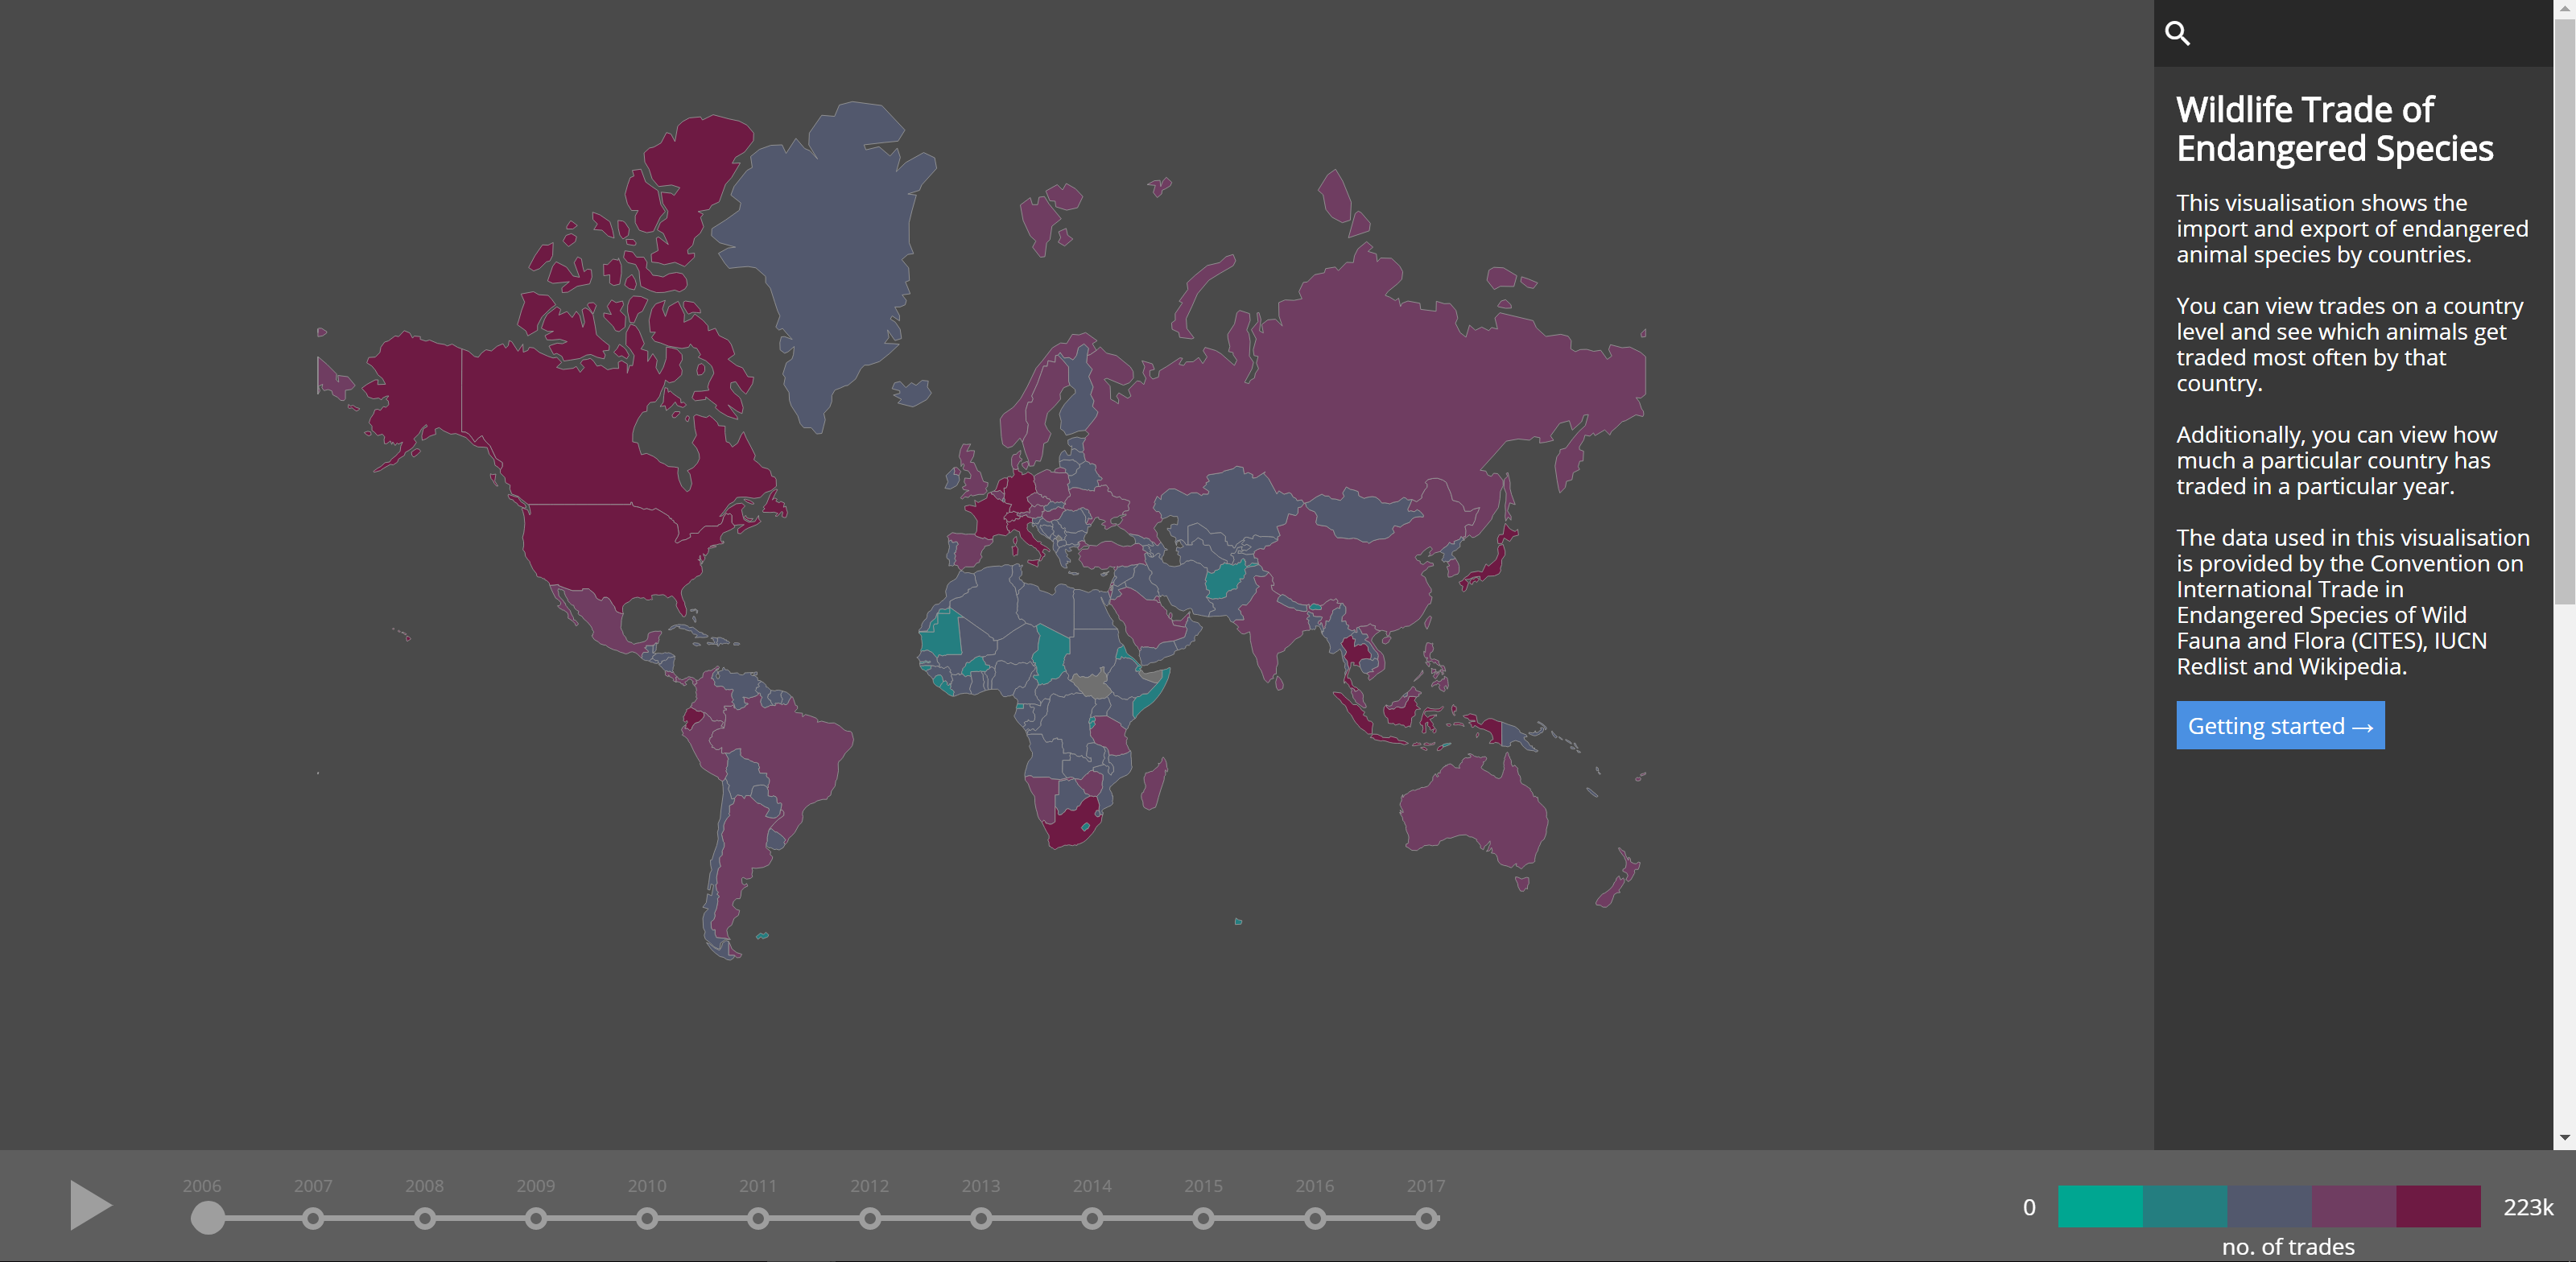
\includegraphics[width=8cm]{images/vis_main.png}
\caption{Main view of the visualization}
\label{vis_main_img}
\end{figure}

\subsection{Visualization}
Users are introduced to the visualization by means of two slides that each contain a single powerful sentence (Figure \ref{vis_intro_img}). The visualization is centered around a world map using the Mercator projection. The map represents the number of trades a particular country has performed using a choropleth map (Figure \ref{vis_main_img}). Based on the number of trades a country has been involved in, the country will be assigned a certain color based on a scale. The scale is dynamically adjusted depending on the highest number of trades in the current selection of the dataset. The different scales are represented in a legend which enables the user to perceive whether a color is an indication of a high or low number of trades. In addition to the choropleth map, the world map also shows which particular countries have traded using connection arches. If the total amount of trades within the current selection has a high volume, the opacity of the arches is slightly lowered in order to reduce clutter. By lowering the opacity, the connections between countries are still distinguishable, even if they overlap one another. 


\subsubsection{Filtering}
The visualization offers several options for the user to manipulate the data shown on the map. The first option is the timeline. The default view of the map contains data from 10 years (Figure \ref{vis_main_img}). By using the timeline, the user can implicitly filter the data and show data from one particular year. Additionally, the user can view how trades have evolved over time by playing the timeline. If the user plays the timeline, the data automatically gets updated for each new year. The second option to manipulate the data shown is by clicking on a country on the world map. This will only show trades performed by the country selected. Aside from showing data on a country level, the user is also able to show data on a species level, where only trades for a specific species are shown. Additionally, the user can combine aforementioned filters in order to see trades by a specific country regarding a species.

\subsubsection{Context \& Exploration}
The sidebar displays information depending on the state or selected filters. For example, if the user is viewing data about a specific species, the sidebar will display information about that species, such as the name, an image, and the endangerment status. This provides context for the currently selected species. The sidebar can also be used in order to find species a user might be interested in or to suggest species which are not yet known to a user. 

\section{Dataset} \label{data}
The visualization uses a dataset extracted from the CITES database\footnote{\url{http://www.iucnredlist.org}, Accessed 23-03-2018} to visualize trades on the map. The structure of the dataset can be found in appendix \ref{tbl:dataset-fields}. 

The CITES dataset was mapped to the choropleth map through \mbox{ISO-3166-1} country codes. These country codes have subsequently been used to identify countries on the map and visualize the data accordingly. Ambiguous country codes (such as SU for USSR) have been removed from the dataset and are not shown in the visualization. 
Originally, the dataset includes entries for all endangered wildlife, including flora. However, rows concerning \textit{flora} have been excluded from the visualization. The color scale of the choropleth map is determined by the country that is involved in the largest number of trades; either export or import. In order to show the connection lines between countries, centroids for every country have been calculated. The centroids serve as the origin and end of a connection line, meaning that all lines start and end at the same point in a country. For every pair of countries, one connection line exists meaning that even if there are multiple trades, they are represented by a single connection line. 
The dataset extracted from the CITES database has also been used to query Wikipedia and Wikidata and provide detailed information about a selected species or country. By using the Latin name of a species or a specific country's name as a query, detailed information (such as a species endangerment status or image) could be retrieved and displayed in the sidebar. 

\section{Design} \label{design}
In this section, the various design decisions that were made during the design process on different levels are discussed. 

\subsection{Interaction Design} \label{InteractionDesign}
Yi et al. \cite{Yi2007} define seven categories with respect to user interaction with an information visualization: \textit{Select, Explore, Reconfigure, Filter, Connect, Encode, and Abstract/Elaborate}. These categories are concerned with the intent of a user when interacting with a system. Based on these categories several design decisions were made.

\textit{Selecting} means that users can select data item(s) they are interested in. In the proposed visualization the user can select a year, species, country or any combination of these parameters. Selecting one or more parameters allows for the user to track any preferred combination. When a single \textbf{species} is selected, the visualization shows how much trades have been made that involved the selection and which countries contributed the most in a certain year (Figure \ref{visid1}). The arcs on the map indicate which countries have participated in these trades. When a single \textbf{country} is selected, the visualization maps shows how much the selected country participated in a certain year. The arcs on the map indicate with which other countries these trades were carried out. When \textbf{both a species and a country} are selected, the visualization indicates with which other countries the selected country has traded the selected species in the selected year (Figure \ref{visid2}). 

\begin{figure} [h] 
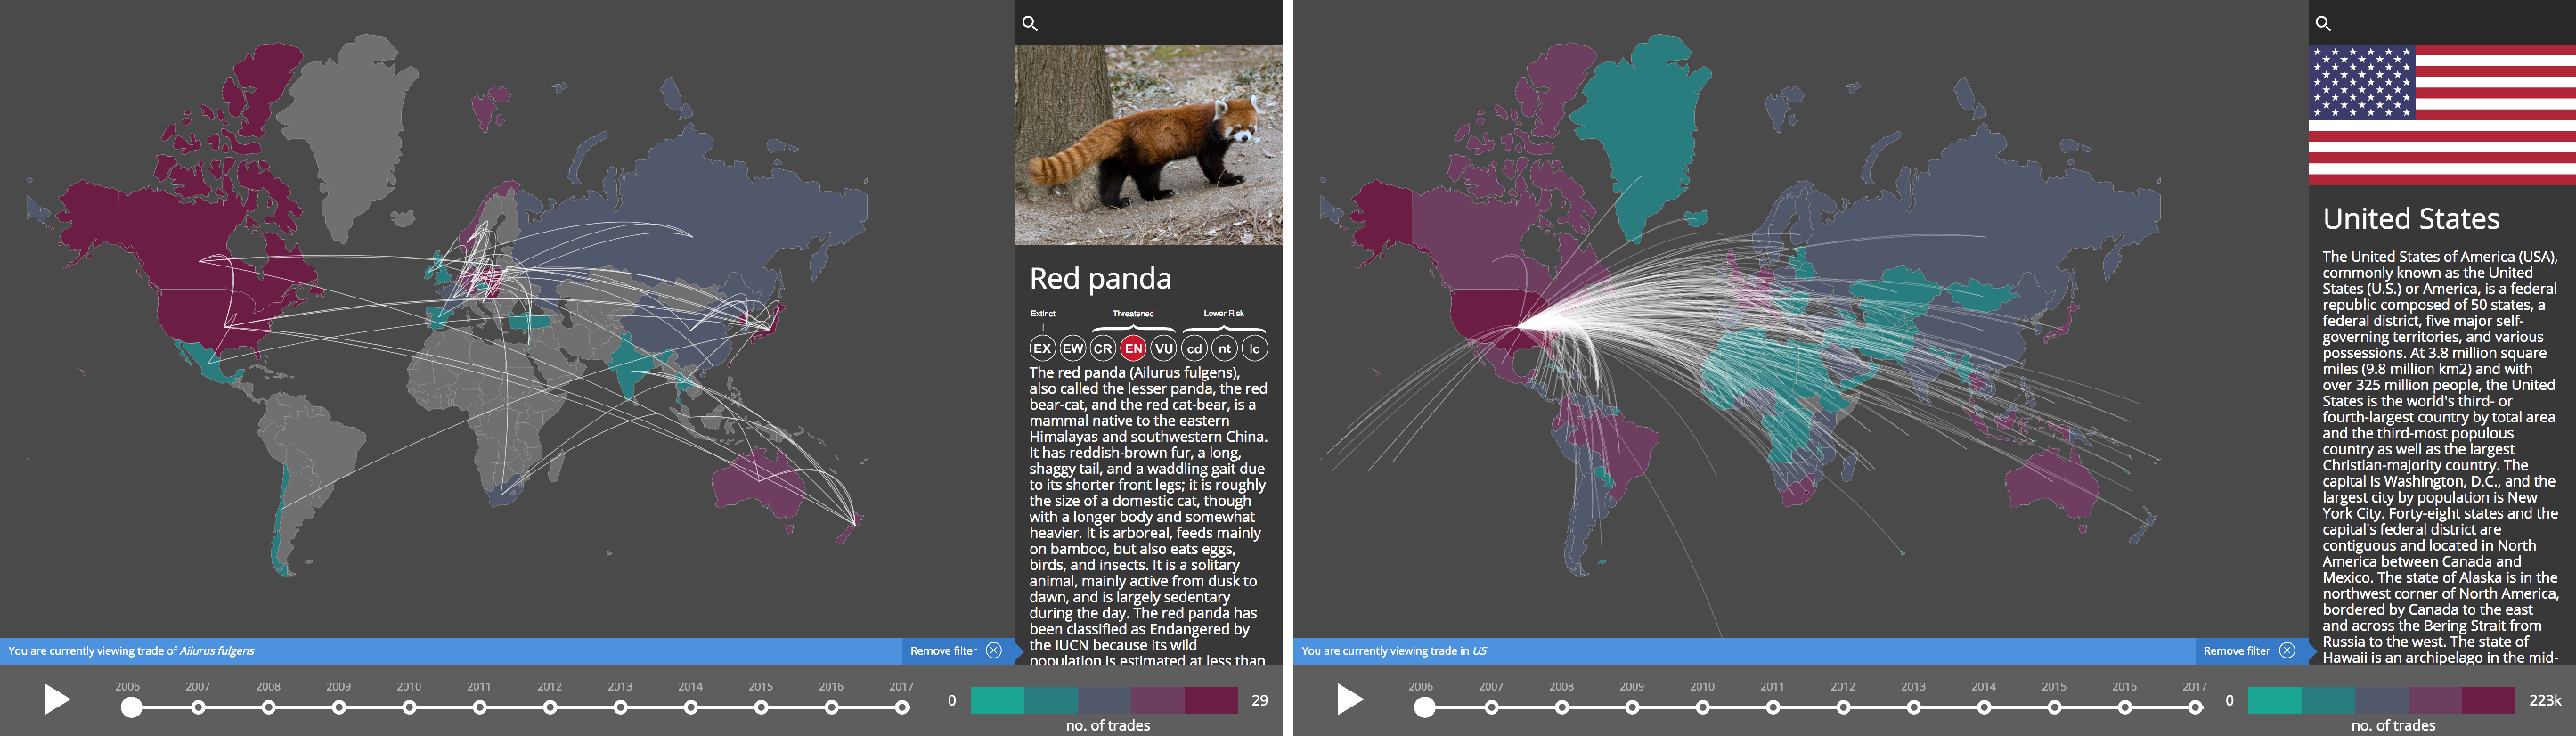
\includegraphics[width=12cm]{images/twosingle.png}
\caption{Left: single species view. Right: single country view}
\label{visid1}
\end{figure}

\textit{Exploration} allows a user to investigate a different set of data cases \cite{Yi2007}. In this category, new data items are usually added or removed. Selecting a species, country or both does not change the view of the map (i.e. it remains the same map). However, it changes the view of the sidebar and the height of the scale in the legend. When a \textbf{species} is selected, the sidebar shows the following information: (a) photo of species, (b) English name, (c) status of endangerment, (d) practical information about the animal, and (e) referral to the corresponding Wikipedia page. When a \textbf{country} is selected, the sidebar shows the flag of the country and its factual information. Also, species are suggested to the user when the search bar is focused.

\textit{Reconfiguration} shows the user a different arrangement or alignment, allowing for different perspectives on the data. It allows hidden data to reveal itself and shows relationships. When the user clicks the play button at the bottom of the screen, the animation connected to the timeline from 2007 until 2017 starts playing. The user can view the trades in the corresponding year. If a \textbf{species} or \textbf{country} is selected, the visualization will be based on the respective selection. If \textbf{both a species and a country} are selected, the visualization will be based on the species in relation to the country.  

\textit{Filtering} allows the user to change the set of data items that are presented. The user defines certain criteria, and only data items that match these constraints will be shown. Different species can be looked up by the user for filtering. When the user clicks on the input field, suggestions are presented. The user can also start typing either the English name or the Latin name. The results are automatically narrowed down and the user can select the preferred species. The filters can be removed by clicking on the ``Remove filter'' button.

\textit{Connecting} is used to place an emphasis on the relationships in the data. When the user first views the visualization, a choropleth map is presented. When a user selects countries or filters a species, not only does the choropleth map change, but an additional layer is added on top of the map showing the connections between countries who have traded.

\textit{Encoding} changes the way the data is presented to the user. Examples of changes within this category are shape, color, and size. The current version does not allow the user to change the encoding of the data. However, a future version could incorporate this by using the sidebar for different types of encodings, such as a line graph or a histogram. 

\textit{Abstraction/Elaboration} gives the user the ability to expand, or abstract the data. When the user views the visualization, all the trades over 10 years are presented. The user can choose to only view the trades of one year, per species or per country. In the data itself, this category is not used, but the user is referred to Wikipedia pages of both species and countries if more information is desirable. 

\subsection{Evaluation Design}
According to North \cite{North2006}, testing on benchmark tasks is the primary method for visualization evaluation. For that reason, a benchmark test would be best used for evaluating the proposed visualization. Users would be asked to perform the following tasks: 
\begin{enumerate}
\item Follow the trade of the Red Panda throughout the available years
\item Find out how much trades involving the Przewalski Horse took place in 2014
\item Follow the trade of the United States throughout the available years
\item Find out which countries traded the most in 2012
\item Follow the trade of the Red Panda in the United States throughout the available years
\end{enumerate}
All of these tasks have to be completed within one minute. The main focus of the test will be on the understandability of the visualization. Because the user has a lot of freedom, it is important to make sure the visualization is clear.

Task 1, 3 and 5 will test if the user \textbf{understands} how to search for a species and country, and how to use the timeline. The output for these tasks is not a specified answer, but rather if they were able to complete the task.

Task 2 and 4 focus on the \textbf{assessment} of the user, if they can find the information to make connections, for example: ``Is it possible to determine which country contributed the most to the trade in a certain year?'' The output for these tasks is: for task 2 a number, and for task 4 a list of countries.

\subsection{Visual Analytics Design}
This section provides a description of the proposed visualization in terms of the \textit{Visual Analytics process} by Keim et al. \cite{Keim2008}. This process (Figure \ref{VAP_Keim}) emphasizes the interaction between data, visualization, model(s) about the data and the user in order to reach the goal of knowledge acquisition (Figure \ref{VAP_Keim}, E.). As discussed in section \ref{data}, the CITIES \textit{data set} was chosen as the basis for the visualization. Pre-processing (Figure \ref{VAP_Keim}, A.) consisted of: linking the scientific Latin names of species, removing non-animal entries, enriching abbreviations with labels, establishing a common relational schema, and, removing trades with incoherent ISO codes. Hereafter, the data was mapped to the visualization through the ISO-3166-1 codes as mentioned in section \ref{data}. The data is filtered based on active parameters, therefore a specific data mining technique (Figure \ref{VAP_Keim}, C.) was not used. In order to reach the goal of knowledge acquisition, the user is capable of interacting (Figure \ref{VAP_Keim}, D.) with the visualization in various ways. The possible interactions only affect the visualization and have no influence with regard to the model. Hence the proposed visualization can be categorized as a \textit{black-box integration} \cite{BertiniInvestigatingDiscovery} in which the user can play around with the parameters. Changes in the parameters are immediately revealed in the visualization. 

\begin{figure} [h]
\centering
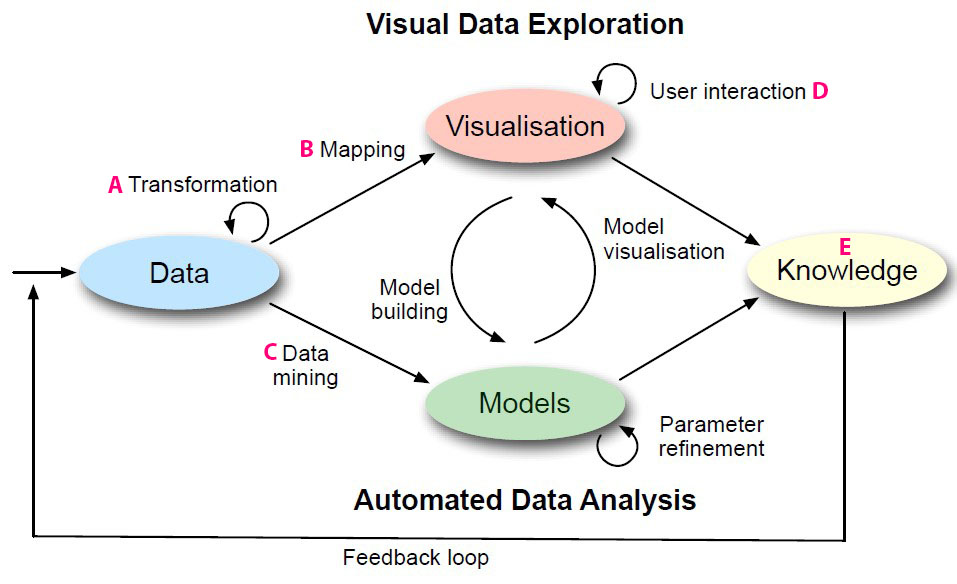
\includegraphics[width=10cm]{images/keim.jpg}
\caption{The Visual Analytics Process by Keim et al. \cite{Keim2008}}
\label{VAP_Keim}
\end{figure}

Because of the \textit{black-box integration} nature of the proposed visualization, user interaction with different parameters does not influence the model behind it. By extending the current system to allow for a \textit{white-box integration} \cite{BertiniInvestigatingDiscovery} in which interactions do influence the model, new insights may be revealed to both the user and the analyst. Another limitation of the proposed visualization is the lack of feedback. Due to the finalization of the project underlying the proposed visualization, feedback generated through the use/testing of the system is not taken into account with regard to the improvement of the model and visualization. Using other relevant datasets and extending the filter possibilities could create deeper levels of insights. 

\subsection{Storytelling Design}
The main goal of the visualization is to give the user insight into the trade of endangered animal species by providing objective, factual information about trading and species. The visualization is presented to the user as an author-driven story using the Martini Glass approach \cite{Segel2010}. When the user views the visualization for the first time, an overlay with introductory text is presented. The text serves the purpose to create awareness about wildlife trade and its influence on the extinction of animal species. Subsequently, the different functionalities of the visualization are explained. After the introduction, the visualization becomes reader driven. From this point onwards, the user is free to explore the visualization. There is no set narrative anymore, displayed information depends on user-made selection. It could be argued that a drill-down approach is used due to the freedom a user has when interacting with the visualization. However, because of the introductory story, a Martini Glass approach is more appropriate. 

\subsection{Visual Thinking Design}
\textit{Visual Thinking} is the process of perceiving the world through visual queries. Humans carry out visual queries for every cognitive task in everyday life. Visual queries can be influenced by properties of the environment that stand out. Ware \cite{Ware2005,Ware2008VisualDesign} discusses four \textit{pre-attentive} properties that should be accounted for when designing visualizations. Pre-attentive properties have the ability to make certain features of visualizations \textit{pop-out}, thus being recognized by the perceptual system before a user is consciously aware of them. 

The first pre-attentive property used to produce a pop-out effect in the proposed visualization is \textbf{Color}. It is mainly used to indicate where on the scale of \textit{total trades made} a certain country falls and to amplify the side- and search bar. The background of the map visualization is assigned the hexadecimal color \#4a4a4a. Countries without trades are assigned the hexadecimal color \#707070, they are only assigned this color when a certain filter does not apply to them. The sidebar was given a slightly darker color than the background of the map, hexadecimal \#383838 to make a clear distinction without standing out too much. The same applies to the search bar with hexadecimal \#282828. These colors, along with the color palette used for the total number of trades scale that applies to the choropleth map, can be seen in figure \ref{colorimg}. The color palette is checked for use in the case of colorblindness with the use of the color-blind simulator and contrast checker \textit{Stark}\footnote{\url{http://www.getstark.co/}, Accessed 27-03-2018}. 

\begin{figure} [h]
\centering
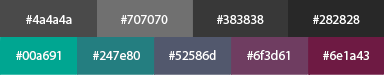
\includegraphics[width= 8cm]{images/colors.png}
\caption{The used colors and their corresponding hexadecimals with regard to the proposed visualization}
\label{colorimg}
\end{figure}

The second pre-attentive property used in the proposed visualization is \textbf{shape}. The 'bubbles' in the time-slider (Figure \ref{slideimg}) are used to give the user a visual clue of the current active year. The size of the time-slider and play-button is based on visibility and as an indicator of importance. The thickness of the trade-arcs is based on a self-deployed exploratory assessment of visibility, distinguishability, and consistency. 

\begin{figure} [h]
\centering

\includegraphics[width= \linewidth]{images/slider.PNG}
\caption{The time-slider used in the proposed visualization}
\label{slideimg}
\end{figure}

The third pre-attentive property used in the proposed visualization is \textbf{motion}. Motion is used to introduce the story behind the visualization, two sentences appear after each other before showing the visualization interface. In a typewriter-like manner, the sentences are displayed to the user. Using motion in this way grabs the user's attention and transfers a sense of seriousness with regard to the subject. Moreover, motion was applied to the placement of the trade arcs. Depending on the nature of a trade, the arc is drawn from or to the selected country to indicate import or export. When a user deploys the play-mode the arcs are re-generated with the transition of every year. A more fluid transition was left out due to high computational costs that disturbed the visualization. The arcs are placed on the centroids of each country due to the lack of a precise geographical location or city within the import or export country. The use of a loading motion indicates to the user that the visualization is loading the requested content.

The final pre-attentive property used in the proposed visualization is \textbf{spatial positioning}. By only using two bars for interaction, the visualization stays clean and grants the user an uncluttered overview. This adds to the transfer of awareness with regard to legal wildlife trade. 


\subsubsection{Enhancing Cognition}

According to Thomas et al. \cite{Thomas2005}, visual analytics systems have the capability to enhance human cognition in six basic ways. Multiple design decisions were made to facilitate the enhancement of human cognition for the proposed visualization. 
By providing the user with a clean interface in which a lot of information is stored in the condensed form of a map and allowing the user to analyze the data on different levels (country, animal, and combination), the visualization increases cognitive resources. 

The visualization does not need symbolic data labels to explicitly code the relation between different data and therefore reduces search. Another way in which the visualization reduces search is by: grouping together data concerning the amount of trades per country between 2006-2017, grouping together data concerning the amount of trades per endangered species between 2006-2017, indicating the endangerment status of individual animal species as per IUCN Red List, and showing information with regard to different countries and animal species as communicated by the corresponding Wikipedia page. 

The visualization also enhances the recognition of patterns for its users. The user does not have to actively specify a query in the visualization but is encouraged to explore the data by interacting with different countries or the search bar. Furthermore, the visualization simplifies the data and only emphasizes certain important aspects of the data (e.g. amount of trades, species traded, countries involved in trading) while hiding less important information (e.g. plant species, incoherent ISO codes, taxonomic information). Lastly, the visualization organizes the data by time, country and species. 

The visualization supports the perceptual inference of relationships through the use of arcs and the filter combination of countries and animal species. By showing changes in trades over time and by using computational power to compute the position of the arcs, relationships are shown that are otherwise more difficult to induce. 

The visualization allows for perceptual monitoring by allowing the user to track a large number of events in the past. However, the visualization does not support the exploration of possible trends in events in the future. Finally, the visualization can be categorized as a manipulable medium since the user can interact with its different components. 

\section{Scientific Excellence} \label{science-excel}
The goal of the visualization is to provide the user with insight into the legal trade of endangered wildlife species. This section describes how a user acquires insight based on the five characteristics as defined by North \cite{North2006}:\textit{complex, deep, qualitative, unexpected and relevant}. 
% The goal of the visualization was to give the user insight into the legal trade of endangered wildlife species. That is why we place an emphasis on insight in this section. Insight has five characteristics, \textit{complex, deep, qualitative, unexpected and relevant} \cite{North2006}. 

The visualization meets the \textit{complex insight} characteristic, due to complex relations the data has, and the visualization illustrates. It uses multiple data points to create an interactive visualization. 

The visualization meets the \textit{deep insight} characteristic, due to the multiple layers of information the visualization shows. The choropleth map is the first layer, the second is the arcs and the remaining layers are the information in the sidebar and the graphs per country in the future.

The visualization meets the \textit{qualitative insight} characteristic, due to the objective perspective it provides. There is no clear opinion given to the visualization, so users are able to form their own and draw their own conclusions. 

The visualization meets the \textit{unexpected insight} characteristic, due to the timeline that takes the user on a journey through time in relation to trades. 

The visualization meets the \textit{relevant insight} characteristic, because it is more than analysis of data. The user is encouraged to think about the subject, and the subject's importance is stressed during the introduction.

\section{Reflection} \label{reflection}
The team consists of 5 MSc students from the UvA \textit{Information Studies} master's programme: Human Centered Multimedia (HCM). All things considered, the project has been successfully realized with its intended initial goal. The communication between team members was clear, roles were assigned, deadlines were met and the atmosphere was good. The group itself consists of two developers and three designers (see Table 1 for the division of roles). 
\begin{table}[!ht]
\centering
\begin{tabular}{ l l p{0cm} }
\hline
\emph{Name} & \emph{Roles} \\
\hline
Sanne & mid-term paper, design, final paper  \\ \hline
Marc & mid-term paper, development, final paper  \\ \hline
Maaike & mid-term paper, design, final paper  \\ \hline
Bastian & mid-term paper, development   \\ \hline
Arjen & mid-term paper, design, final paper \\ \hline
\end{tabular}
\caption{Role division during the project} \label{tbl:role-division}
\end{table} 
The division of the group into developers/designers allowed for an iterative development and design approach where the both 'groups' proposed designs, changes, and technical functionalities. Moreover, constant feedback was provided on which decisions were based. Even though this approach allowed for fast iterations and informed decision making, it also revealed a difficulty. At a certain point, it became apparent that it was not entirely clear what the visualization would entail. This occurred because the goal of the visualization was defined too vaguely and decisions up until that point were made on a level that was too global. Subsequently leading to minor difficulties in designing and developing the visualization. In a future project, this should be done sooner and documented more thoroughly to avoid confusion.  












